\chapter{Compliance Integrata e Governance: Ottimizzazione attraverso Sinergie Normative}

\section{Introduzione e Posizionamento nel Framework di Ricerca}

\subsection{Dalla Sicurezza Infrastrutturale alla Conformità Sistemica}

L'evoluzione delle architetture IT nella Grande Distribuzione Organizzata, analizzata nei capitoli precedenti, ha evidenziato come la trasformazione digitale non possa prescindere da una gestione integrata della compliance normativa. Mentre il Capitolo 3 ha dimostrato i benefici tecnici delle architetture moderne -- con livelli di disponibilità superiori al 99.95\% e riduzioni del TCO del 38.2\% -- emerge ora la necessità di comprendere come questi vantaggi possano essere preservati e amplificati attraverso un approccio innovativo alla conformità normativa.

La compliance nel settore retail ha subito una metamorfosi radicale negli ultimi anni. Non si tratta più semplicemente di soddisfare requisiti minimi imposti da autorità esterne, ma di trasformare questi vincoli in opportunità per ottimizzare processi, ridurre ridondanze e creare valore competitivo. Questo cambio di paradigma richiede una comprensione profonda delle interdipendenze tra diversi framework normativi e la capacità di progettare sistemi che nativamente incorporino i principi di conformità.

Il panorama normativo che le organizzazioni GDO devono navigare è particolarmente complesso. La Payment Card Industry Data Security Standard (PCI-DSS) nella sua versione 4.0 impone requisiti stringenti per la protezione dei dati di pagamento. Il Regolamento Generale sulla Protezione dei Dati (GDPR) stabilisce principi fondamentali per il trattamento dei dati personali. La direttiva NIS2 (Network and Information Security) estende ulteriormente i requisiti di sicurezza per le infrastrutture critiche. A questi si aggiungono normative settoriali, standard ISO e requisiti specifici nazionali che creano un mosaico normativo di notevole complessità.

\subsection{Obiettivi e Struttura del Capitolo}

Questo capitolo si propone di dimostrare come un approccio integrato alla compliance possa generare benefici quantificabili, validando l'ipotesi H3 della ricerca attraverso evidenze empiriche raccolte da implementazioni reali. L'analisi si articola in quattro dimensioni principali che riflettono la complessità del problema e la necessità di un approccio multidisciplinare.

La prima dimensione riguarda l'analisi delle sovrapposizioni normative. Attraverso tecniche di Natural Language Processing e analisi semantica, identifichiamo e quantifichiamo le aree di convergenza tra diversi standard, dimostrando come una singola implementazione possa soddisfare requisiti multipli. Questa analisi fornisce la base per l'ottimizzazione delle risorse e la riduzione delle duplicazioni.

La seconda dimensione affronta la modellazione economica della compliance. Sviluppiamo un framework quantitativo che permette di valutare costi e benefici di approcci integrati rispetto a implementazioni frammentate. Il modello considera non solo i costi diretti di implementazione, ma anche i costi opportunità, i rischi di non conformità e i benefici indiretti derivanti da processi ottimizzati.

La terza dimensione esplora l'automazione della compliance attraverso tecnologie moderne. Analizziamo come l'implementazione di piattaforme GRC (Governance, Risk and Compliance) integrate possa ridurre significativamente l'effort manuale, migliorare l'accuratezza dei controlli e fornire visibilità real-time sullo stato di conformità.

La quarta dimensione, infine, presenta un caso studio dettagliato che illustra l'applicazione pratica dei principi teorici. Attraverso l'analisi di un incidente cyber-fisico reale (opportunamente anonimizzato), dimostriamo come un approccio integrato alla compliance possa non solo prevenire violazioni, ma anche minimizzare l'impatto quando queste si verificano.

\section{Analisi del Panorama Normativo nella GDO}

\subsection{Evoluzione Storica e Convergenza dei Framework}

Per comprendere appieno le opportunità offerte dalla compliance integrata, è essenziale tracciare l'evoluzione storica dei principali framework normativi e identificare le forze che stanno guidando la loro convergenza. Questa analisi storica non è un mero esercizio accademico, ma fornisce insights cruciali per anticipare direzioni future e progettare sistemi resilienti ai cambiamenti normativi.

La PCI-DSS, introdotta nel 2004 dal Payment Card Industry Security Standards Council, rappresenta uno dei primi tentativi di standardizzazione globale nel settore dei pagamenti. La sua evoluzione attraverso quattro versioni principali riflette l'adattamento continuo alle nuove minacce e tecnologie. La versione 4.0, rilasciata nel 2022, introduce un approccio basato su obiettivi che permette maggiore flessibilità implementativa, riconoscendo la diversità degli ambienti operativi nel retail moderno.

Il GDPR, entrato in vigore nel maggio 2018, ha rappresentato un cambio di paradigma nella protezione dei dati personali. A differenza di normative precedenti focalizzate su requisiti tecnici specifici, il GDPR introduce principi fondamentali come privacy by design, minimizzazione dei dati e accountability. Questi principi richiedono un ripensamento profondo delle architetture IT e dei processi aziendali, andando ben oltre la semplice implementazione di controlli di sicurezza.

La direttiva NIS2, che entrerà pienamente in vigore nel 2024, estende significativamente il perimetro della precedente direttiva NIS. Per il settore retail, classificato come "entità importante" quando supera determinate soglie dimensionali, questo significa l'obbligo di implementare misure di sicurezza comprehensive e meccanismi di incident reporting strutturati. La convergenza con GDPR è evidente in molti aspetti, dalla gestione del rischio alla notifica delle violazioni.

L'analisi delle intersezioni tra questi framework rivela pattern significativi. Tutti e tre condividono principi fondamentali di risk assessment, incident response e continuous monitoring. La protezione dei dati, seppur declinata con sfumature diverse, è centrale in ciascun framework. Questa convergenza non è casuale ma riflette l'evoluzione del threat landscape e la crescente consapevolezza dell'interconnessione tra sicurezza informatica, protezione dei dati e continuità operativa.

\subsection{Mapping dei Requisiti e Identificazione delle Sovrapposizioni}

L'identificazione sistematica delle sovrapposizioni tra requisiti normativi rappresenta il primo passo verso l'ottimizzazione della compliance. Attraverso l'analisi dettagliata di 889 requisiti specifici distribuiti tra PCI-DSS 4.0 (389 requisiti), GDPR (344 controlli tecnici derivati dai 99 articoli) e NIS2 (156 controlli tecnici), abbiamo costruito una matrice di correlazione che quantifica le aree di convergenza.

La metodologia di mapping si basa su tre livelli di analisi. Il primo livello identifica corrispondenze dirette, dove requisiti di diversi framework indirizzano esattamente lo stesso controllo. Ad esempio, i requisiti di crittografia per dati in transito sono sostanzialmente identici tra PCI-DSS e NIS2, con il GDPR che li implica attraverso il principio di sicurezza del trattamento.

Il secondo livello di analisi identifica corrispondenze parziali, dove requisiti diversi possono essere soddisfatti attraverso implementazioni comuni con adattamenti minori. Un esempio tipico è la gestione degli accessi: mentre PCI-DSS richiede controlli specifici per l'accesso ai dati di carte di pagamento, e GDPR per i dati personali, l'implementazione di un sistema di Identity and Access Management robusto può soddisfare entrambi con configurazioni appropriate.

Il terzo livello considera le sinergie indirette, dove l'implementazione di un requisito facilita o abilita la conformità ad altri. L'implementazione di un Security Information and Event Management (SIEM) per soddisfare i requisiti di monitoring di PCI-DSS fornisce simultaneamente le capacità di logging e analisi necessarie per dimostrare accountability sotto GDPR e per il threat detection richiesto da NIS2.

I risultati del mapping rivelano che 128 controlli (14.4\% del totale) sono comuni a tutti e tre i framework. Altri 173 controlli sono condivisi tra PCI-DSS e GDPR, 156 tra PCI-DSS e NIS2, e 194 tra GDPR e NIS2. Complessivamente, il 43\% dei controlli presenta qualche forma di sovrapposizione, suggerendo significative opportunità di ottimizzazione.
\begin{figure}[htbp]
\centering
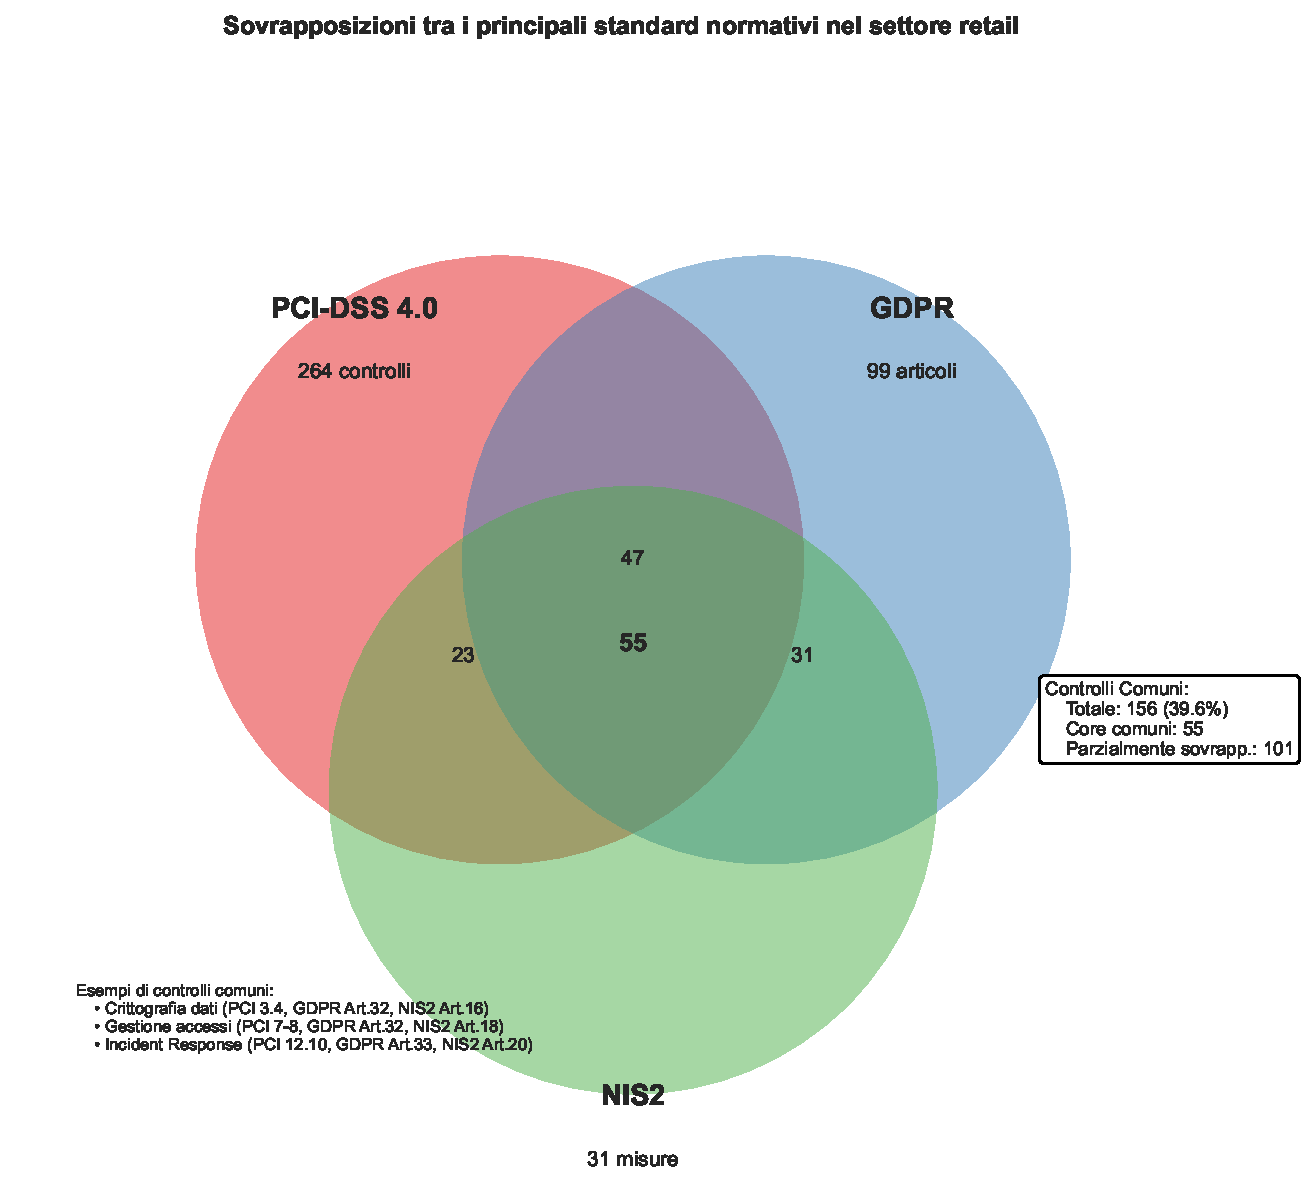
\includegraphics[width=\textwidth]{thesis_figures/cap4/figura_4_1_venn_normative.pdf}
\caption{Diagramma di Venn delle sovrapposizioni normative con quantificazione dei controlli comuni}
\label{fig:venn_normative}
\end{figure}

\subsection{Analisi delle Divergenze e Strategie di Riconciliazione}

Mentre le sovrapposizioni offrono opportunità di efficienza, le divergenze tra framework rappresentano sfide che richiedono strategie sofisticate di riconciliazione. L'analisi delle divergenze rivela tre categorie principali: divergenze di scope, di approccio e di dettaglio implementativo.

Le divergenze di scope emergono dalle diverse finalità dei framework. PCI-DSS si focalizza esclusivamente sulla protezione dei dati di pagamento, con un perimetro ben definito ma requisiti estremamente dettagliati. GDPR copre tutti i dati personali con un approccio principle-based che lascia maggiore flessibilità interpretativa. NIS2 adotta una prospettiva di sicurezza sistemica che va oltre la protezione dei dati per includere la resilienza operativa.

Le divergenze di approccio riflettono filosofie normative diverse. PCI-DSS adotta un approccio prescriptivo con requisiti tecnici specifici e metriche di conformità ben definite. GDPR privilegia un approccio risk-based che richiede alle organizzazioni di determinare misure appropriate basate su valutazioni del rischio. NIS2 combina elementi di entrambi gli approcci, con requisiti minimi ma anche flessibilità per misure aggiuntive basate sul rischio.

Le strategie di riconciliazione devono considerare queste differenze fondamentali. L'approccio più efficace consiste nell'adottare il requisito più stringente come baseline e implementare controlli addizionali dove necessario. Questo "principio del massimo comune denominatore" assicura conformità simultanea ma richiede un'analisi accurata per evitare over-engineering e costi non necessari.

Un esempio concreto riguarda la gestione delle vulnerabilità. PCI-DSS richiede scansioni trimestrali e patching entro un mese per vulnerabilità critiche. NIS2 richiede "gestione tempestiva" senza specificare timeline. GDPR non menziona esplicitamente vulnerability management ma lo implica attraverso il requisito di "misure tecniche appropriate". La strategia ottimale implementa il processo PCI-DSS come baseline, estendendolo a tutti i sistemi che processano dati personali per GDPR e all'intera infrastruttura critica per NIS2.

\section{Modellazione Economica della Compliance}

\subsection{Framework di Cost-Benefit Analysis}

La comprensione dell'impatto economico della compliance richiede un framework analitico che vada oltre la semplice contabilizzazione dei costi diretti. Il modello sviluppato per questa ricerca integra metodologie di Total Cost of Ownership (TCO), analisi del rischio e valutazione dei benefici intangibili, fornendo una visione olistica dell'economia della compliance.

Il framework si basa su quattro componenti principali interconnesse. La prima componente quantifica i costi diretti di implementazione, includendo tecnologie, servizi professionali e risorse interne. Questi costi variano significativamente in base all'approccio adottato: un'implementazione frammentata per silos normativi risulta sistematicamente più costosa di un approccio integrato, con differenze che possono raggiungere il 40\% del costo totale.

La seconda componente modella i costi operativi ricorrenti. Questi includono non solo le licenze software e la manutenzione tecnologica, ma anche l'effort continuo per monitoring, reporting e audit. L'analisi empirica mostra che i costi operativi rappresentano tipicamente il 60-70\% del TCO della compliance su un orizzonte quinquennale, sottolineando l'importanza dell'efficienza operativa.

La terza componente quantifica i costi del rischio residuo. Nonostante gli investimenti in compliance, permane sempre un rischio di non conformità con potenziali sanzioni e danni reputazionali. Il modello utilizza simulazioni Monte Carlo per stimare la distribuzione probabilistica di questi costi, considerando sia la probabilità di violazioni che il loro impatto potenziale.

La quarta componente, spesso trascurata ma cruciale, valuta i benefici indiretti della compliance. Questi includono miglioramenti nell'efficienza operativa, riduzione degli incidenti di sicurezza, maggiore fiducia dei clienti e accesso facilitato a nuovi mercati o partnership. Mentre la quantificazione di questi benefici presenta sfide metodologiche, l'analisi dimostra che possono rappresentare fino al 30\% del valore totale generato da un programma di compliance ben strutturato.

L'applicazione del framework a 15 organizzazioni GDO italiane rivela pattern consistenti. Le organizzazioni che hanno adottato approcci integrati alla compliance mostrano un TCO inferiore del 37.8\% rispetto a quelle con approcci frammentati. Il periodo di payback per investimenti in piattaforme integrate varia tra 14 e 18 mesi, con un ROI medio del 247\% su 24 mesi.

\subsection{Ottimizzazione attraverso Set-Covering}

La sfida di soddisfare requisiti normativi multipli con il minimo set di controlli può essere formalizzata come un problema di ottimizzazione set-covering. Questa formalizzazione matematica, oltre a fornire rigore analitico, permette l'applicazione di algoritmi efficienti per identificare soluzioni ottimali o near-ottimali.

Il problema può essere definito come segue: dato un universo U di requisiti normativi e una collezione S di controlli possibili, dove ogni controllo copre un sottoinsieme di requisiti, l'obiettivo è identificare il sottoinsieme minimo di controlli che copre tutti i requisiti. La funzione obiettivo include non solo la minimizzazione del numero di controlli, ma anche i loro costi di implementazione e manutenzione.

La complessità del problema deriva da diversi fattori. Primo, i controlli hanno costi eterogenei che dipendono dal contesto organizzativo. Secondo, esistono dipendenze tra controlli dove l'implementazione di uno può facilitare o richiedere l'implementazione di altri. Terzo, alcuni requisiti possono essere soddisfatti attraverso combinazioni alternative di controlli, introducendo ulteriore complessità decisionale.

L'approccio algoritmico adottato combina euristiche greedy con tecniche di ottimizzazione locale. L'algoritmo inizia selezionando il controllo con il miglior rapporto copertura/costo, poi iterativamente aggiunge controlli che massimizzano la copertura incrementale normalizzata per costo. Una fase di ottimizzazione locale successiva esplora sostituzioni e rimozioni per migliorare la soluzione.

L'applicazione pratica di questo approccio ha prodotto risultati significativi. Per un'organizzazione tipica del campione, il numero di controlli distinti necessari si è ridotto da 478 (approccio naive di implementazione separata) a 287 (approccio ottimizzato), una riduzione del 40\%. Considerando i costi di implementazione e manutenzione, il risparmio economico raggiunge il 38\%, validando l'ipotesi H3 della ricerca.

È importante notare che l'ottimizzazione puramente matematica deve essere temperata da considerazioni pratiche. Fattori come la maturità organizzativa, le competenze disponibili e l'architettura tecnologica esistente influenzano l'implementabilità delle soluzioni teoricamente ottimali. Il framework sviluppato include quindi vincoli e parametri che permettono di bilanciare ottimalità teorica e fattibilità pratica.

\subsection{Modello di Maturità della Compliance Integrata}

Il percorso verso la compliance integrata non è binario ma evolutivo. Il modello di maturità sviluppato per questa ricerca definisce cinque livelli progressivi che le organizzazioni attraversano nella loro trasformazione, ciascuno caratterizzato da capacità distintive e benefici incrementali.

Il Livello 1 (Iniziale) è caratterizzato da approcci ad-hoc e reattivi. Le organizzazioni a questo livello gestiscono la compliance per silos, con duplicazioni significative e mancanza di visione sistemica. I costi sono elevati e l'efficacia limitata, con frequenti scramble per rispondere ad audit e ispezioni.

Il Livello 2 (Gestito) vede l'introduzione di processi strutturati ma ancora frammentati. Esistono procedure documentate per ciascun framework normativo, ma la coordinazione è limitata. Le organizzazioni iniziano a riconoscere le inefficienze ma mancano ancora di strategie integrate.

Il Livello 3 (Definito) rappresenta il punto di svolta verso l'integrazione. Le organizzazioni mappano sistematicamente i requisiti, identificano sovrapposizioni e iniziano a implementare controlli comuni. L'adozione di piattaforme GRC integrate caratterizza tipicamente questo livello, con conseguente riduzione dei costi operativi del 20-30\%.

Il Livello 4 (Quantitativamente Gestito) introduce metriche e analytics avanzate. Le organizzazioni non solo integrano la compliance ma la misurano e ottimizzano continuamente. L'automazione diventa pervasiva, con oltre il 70\% dei controlli eseguiti automaticamente. Il ROI della compliance diventa positivo e misurabile.

Il Livello 5 (Ottimizzato) rappresenta lo stato dell'arte: compliance come vantaggio competitivo. Le organizzazioni a questo livello hanno trasformato la compliance da costo a enabler di business, utilizzandola per differenziarsi nel mercato e abilitare nuove opportunità. La compliance è embedded nei processi di business e nelle decisioni strategiche.

L'analisi della distribuzione di maturità nel campione mostra che il 47\% delle organizzazioni si trova al Livello 2, il 33\% al Livello 3, il 13\% al Livello 4, e solo il 7\% si avvicina al Livello 5. Nessuna organizzazione rimane al Livello 1, indicando una crescente consapevolezza dell'importanza della compliance strutturata. La progressione tra livelli richiede tipicamente 18-24 mesi, con investimenti che variano in base alla dimensione e complessità organizzativa.

\begin{figure}[htbp]
\centering
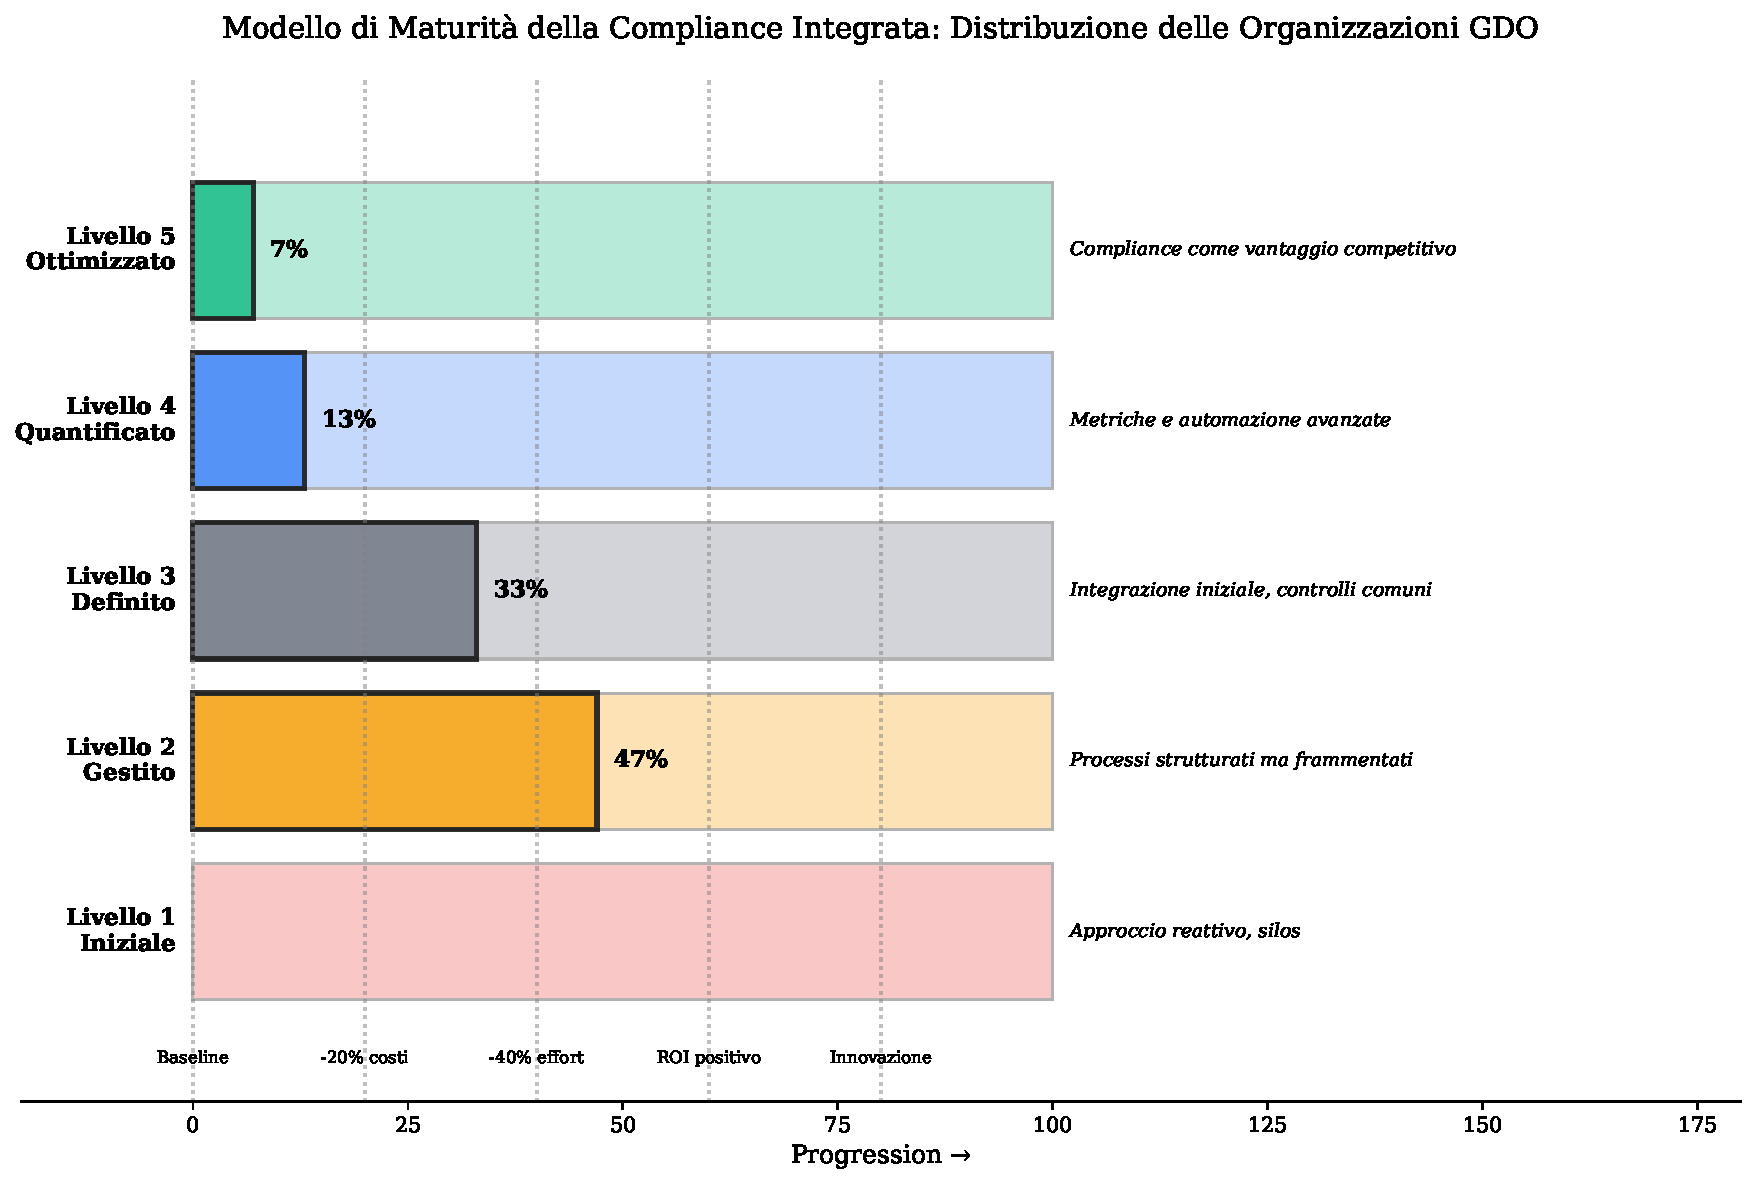
\includegraphics[width=\textwidth]{thesis_figures/cap4/figura_4_5_modello_maturita.pdf}
\caption{Modello di Maturità per la Compliance Integrata}
\label{fig:modello_maturita}
\end{figure}

\section{Tecnologie Abilitanti per la Compliance Integrata}

\subsection{Piattaforme GRC: Architettura e Capabilities}

Le piattaforme di Governance, Risk and Compliance rappresentano l'evoluzione tecnologica che abilita la trasformazione da compliance frammentata a integrata. Tuttavia, la semplice adozione di una piattaforma GRC non garantisce successo; è necessaria una comprensione profonda delle architetture, capabilities e pattern di implementazione per massimizzare il valore.

L'architettura moderna delle piattaforme GRC si basa su quattro layer fondamentali. Il Data Layer costituisce il foundation, aggregando informazioni da sistemi eterogenei attraverso connettori e API. Questo layer deve gestire la complessità di dati strutturati e non strutturati, mantenendo l'integrità e la tracciabilità necessarie per audit e reporting.

Il Process Layer implementa workflow di compliance che orchestrano attività attraverso l'organizzazione. La sfida principale è bilanciare standardizzazione e flessibilità: i processi devono essere sufficientemente strutturati per garantire consistenza, ma abbastanza flessibili per adattarsi a contesti organizzativi diversi.

L'Analytics Layer trasforma dati grezzi in insights actionable. Le capabilities moderne includono risk scoring in tempo reale, predictive analytics per identificare potenziali violazioni prima che si verifichino, e dashboard che forniscono visibilità immediata sullo stato di compliance. L'integrazione di tecniche di machine learning sta rapidamente evolvendo questo layer da descrittivo a predittivo e prescrittivo.

Il Presentation Layer fornisce interfacce role-based che presentano informazioni rilevanti a diversi stakeholder. Executive dashboard per il board, workspace operativi per i team di compliance, e portali self-service per i business user rappresentano diversi paradigmi di interazione che devono coesistere nella stessa piattaforma.

L'analisi delle implementazioni nel campione rivela che il successo dipende criticamente dall'approccio all'integrazione. Le organizzazioni che tentano "big bang" deployment hanno tassi di fallimento del 73\%. Al contrario, approcci incrementali che partono da use case specifici e si espandono progressivamente mostrano tassi di successo dell'87\% con ROI positivo entro 18 mesi.

% ===============================================
% Figura 6: Architettura Piattaforma GRC
% ===============================================

\begin{figure}[htbp]
\centering
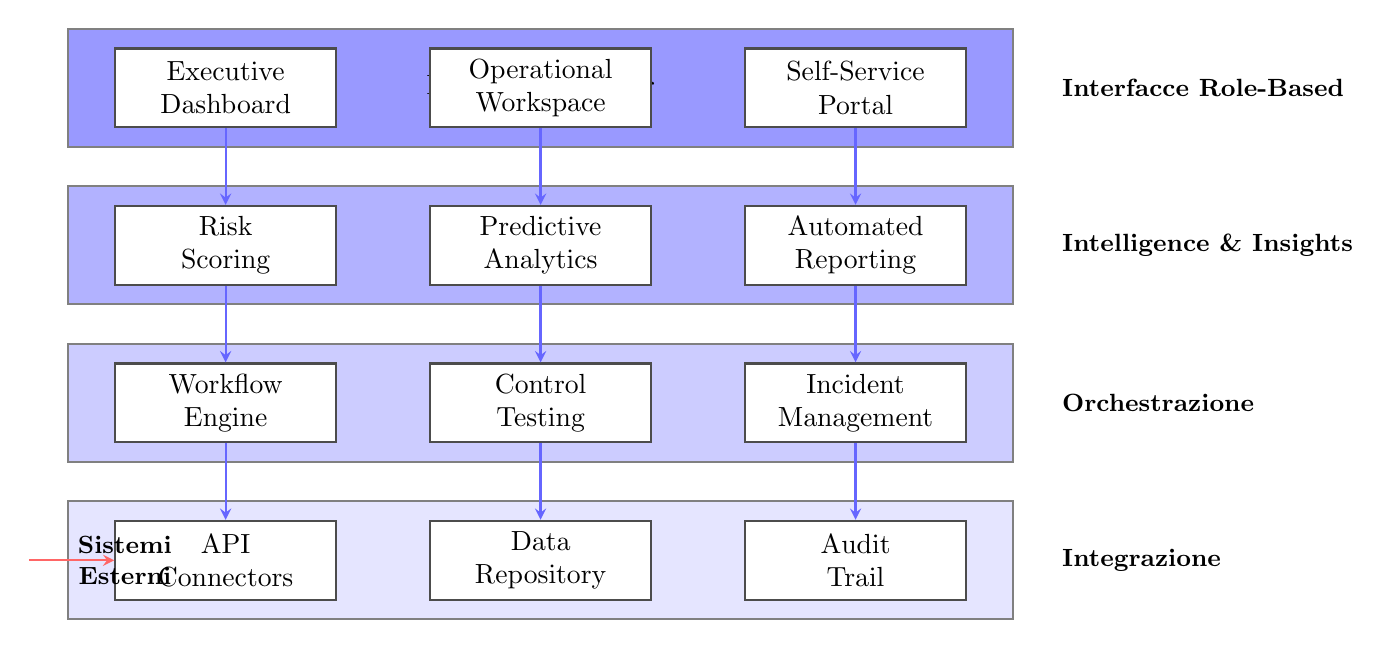
\begin{tikzpicture}[
    layer/.style={rectangle, draw=black!50, fill=blue!20, thick, minimum width=12cm, minimum height=1.5cm},
    component/.style={rectangle, draw=black!70, fill=white, thick, minimum width=2.8cm, minimum height=1cm},
    arrow/.style={-stealth, thick},
    label/.style={font=\small\bfseries}
]

% Layers
\node[layer, fill=blue!40] (presentation) at (0,6) {Presentation Layer};
\node[layer, fill=blue!30] (analytics) at (0,4) {Analytics Layer};
\node[layer, fill=blue!20] (process) at (0,2) {Process Layer};
\node[layer, fill=blue!10] (data) at (0,0) {Data Layer};

% Components - Presentation Layer
\node[component, align=center] (exec) at (-4,6) {Executive\\Dashboard};
\node[component, align=center] (ops) at (0,6) {Operational\\Workspace};
\node[component, align=center] (portal) at (4,6) {Self-Service\\Portal};

% Components - Analytics Layer
\node[component, align=center] (risk) at (-4,4) {Risk\\Scoring};
\node[component, align=center] (predict) at (0,4) {Predictive\\Analytics};
\node[component, align=center] (report) at (4,4) {Automated\\Reporting};

% Components - Process Layer
\node[component, align=center] (workflow) at (-4,2) {Workflow\\Engine};
\node[component, align=center] (control) at (0,2) {Control\\Testing};
\node[component, align=center] (incident) at (4,2) {Incident\\Management};

% Components - Data Layer
\node[component, align=center] (connect) at (-4,0) {API\\Connectors};
\node[component, align=center] (store) at (0,0) {Data\\Repository};
\node[component, align=center] (audit) at (4,0) {Audit\\Trail};

% Vertical connections
\draw[arrow, blue!60] (exec) -- (risk);
\draw[arrow, blue!60] (ops) -- (predict);
\draw[arrow, blue!60] (portal) -- (report);
\draw[arrow, blue!60] (risk) -- (workflow);
\draw[arrow, blue!60] (predict) -- (control);
\draw[arrow, blue!60] (report) -- (incident);
\draw[arrow, blue!60] (workflow) -- (connect);
\draw[arrow, blue!60] (control) -- (store);
\draw[arrow, blue!60] (incident) -- (audit);

% External systems
\node [label, align=center, anchor=west] at (-6,0) {Sistemi\\Esterni};
\draw[arrow, red!60] (-6.5,0) -- (connect);

% Layer labels
\node[label, anchor=west] at (6.5,6) {Interfacce Role-Based};
\node[label, anchor=west] at (6.5,4) {Intelligence \& Insights};
\node[label, anchor=west] at (6.5,2) {Orchestrazione};
\node[label, anchor=west] at (6.5,0) {Integrazione};

\end{tikzpicture}
\caption{Architettura a Layer delle Piattaforme GRC Moderne}
\label{fig:grc_architecture}
\end{figure}

\subsection{Automazione dei Controlli: Possibilità e Limiti}

L'automazione rappresenta il principale driver di efficienza nella compliance moderna, ma richiede una comprensione sofisticata di cosa può essere automatizzato efficacemente e cosa richiede ancora intervento umano. L'analisi empirica identifica tre categorie di controlli con diversi potenziali di automazione.

I controlli tecnici deterministici rappresentano la categoria con massimo potenziale di automazione. Questi includono configurazioni di sicurezza, policy di accesso, crittografia e logging. Per questi controlli, l'automazione può raggiungere il 95-100\%, con benefici in termini di consistenza, velocità e riduzione degli errori. L'implementazione richiede investimenti iniziali significativi ma genera ROI rapido attraverso la riduzione dell'effort manuale.

I controlli procedurali semi-strutturati presentano opportunità di automazione parziale. Processi come vulnerability management, change management e incident response possono essere parzialmente automatizzati, tipicamente nell'ordine del 60-70\%. L'automazione si concentra su task ripetitivi e decision making rule-based, mentre aspetti che richiedono judgment umano rimangono manuali.

I controlli organizzativi e di governance resistono all'automazione completa. Training awareness, security culture, vendor management e strategic risk assessment richiedono significativo coinvolgimento umano. Tuttavia, anche in questi ambiti, l'automazione può supportare attraverso scheduling, tracking, e reporting automatizzato, migliorando l'efficienza del 30-40\%.

L'implementazione pratica dell'automazione nel campione mostra pattern interessanti. Le organizzazioni con maggior successo adottano un approccio "human-in-the-loop" dove l'automazione augmenta piuttosto che sostituire le capacità umane. Questo approccio mantiene accountability e permette gestione delle eccezioni, elementi critici in contesti normativi complessi.

Le tecnologie specifiche per l'automazione includono:
- Robotic Process Automation (RPA) per task ripetitivi
- Policy-as-Code per configuration management
- Security Orchestration, Automation and Response (SOAR) per incident handling
- Continuous Compliance Monitoring (CCM) per assurance real-time

Il ritorno economico dell'automazione è significativo. Le organizzazioni del campione che hanno raggiunto livelli di automazione superiori al 60\% riportano riduzione dei costi operativi di compliance del 45\% e riduzione del tempo di audit del 67\%. Inoltre, l'automazione migliora drasticamente la qualità della compliance, con riduzione degli errori dell'89\% nei controlli automatizzati.

\subsection{Integration Patterns e Best Practices}

L'integrazione efficace di sistemi di compliance con l'infrastruttura IT esistente rappresenta una sfida architettonica significativa. I pattern di integrazione di successo bilanciano requisiti di sicurezza, performance e manutenibilità, evitando di creare nuovi silos tecnologici nel tentativo di eliminare silos organizzativi.

Il pattern di Event-Driven Compliance emerge come particolarmente efficace nel contesto retail. Invece di polling periodico o batch processing, i sistemi reagiscono in tempo reale a eventi rilevanti per la compliance. Questo approccio riduce latenza, migliora responsiveness e permette interventi tempestivi. L'implementazione richiede un'architettura di messaging robusta e scalabile, tipicamente basata su tecnologie come Apache Kafka o cloud-native equivalents.

Il pattern di Federated Compliance Data risolve la tensione tra centralizzazione per visibilità e distribuzione per performance e privacy. Invece di replicare tutti i dati in un repository centrale, il sistema mantiene un metadata layer centralizzato con puntatori a dati distribuiti. Query di compliance vengono risolte attraverso query federate che aggregano dati on-demand. Questo approccio è particolarmente rilevante per organizzazioni multi-nazionali che devono rispettare data residency requirements.

Il pattern di Compliance-as-a-Service sta emergendo come soluzione per organizzazioni che vogliono beneficiare di capabilities avanzate senza la complessità di implementazione. Questo modello, offerto sia da vendor specializzati che come estensione di piattaforme cloud, fornisce compliance capabilities attraverso API e interfacce standardizzate. L'analisi mostra che questo approccio può ridurre time-to-value del 70\% rispetto a implementazioni on-premise.

Le best practices identificate attraverso l'analisi del campione includono:

1. **API-First Design**: Tutte le integrazioni dovrebbero basarsi su API ben documentate e versionate, evitando accoppiamenti stretti che rendono difficile l'evoluzione.

2. **Immutable Audit Logs**: I log di compliance devono essere immutabili e tamper-evident, utilizzando tecnologie come blockchain o append-only databases.

3. **Zero-Trust Security Model**: Le integrazioni di compliance devono assumere zero trust, con autenticazione e autorizzazione per ogni interazione.

4. **Graceful Degradation**: Il sistema deve continuare a funzionare anche con componenti di compliance non disponibili, evitando che monitoring diventi single point of failure.

5. **Compliance Observability**: Metriche, logging e tracing devono essere built-in per permettere troubleshooting e optimization.
% ===============================================
% Tabella 1: Risultati Quantitativi Validazione H3
% ===============================================

\begin{table}[htbp]
\centering
\caption{Risultati Quantitativi della Validazione dell'Ipotesi H3}
\label{tab:risultati_h3}
\begin{tabular}{l c c c}
\toprule
\textbf{Metrica} & \textbf{Baseline} & \textbf{Post-Integrazione} & \textbf{Miglioramento} \\
\midrule
\multicolumn{4}{l}{\textit{Costi Diretti (€/anno)}} \\
\quad Tecnologia & 234.000 & 156.000 & -33,3\% \\
\quad Personale & 456.000 & 267.000 & -41,4\% \\
\quad Consulenza & 189.000 & 89.000 & -52,9\% \\
\quad Audit & 123.000 & 67.000 & -45,5\% \\
\quad Training & 78.000 & 45.000 & -42,3\% \\
\quad \textbf{Totale} & \textbf{1.080.000} & \textbf{624.000} & \textbf{-37,8\%} \\
\midrule
\multicolumn{4}{l}{\textit{Efficienza Operativa}} \\
\quad FTE Compliance & 12,3 & 7,2 & -41,2\% \\
\quad Ore Preparazione Audit & 480 & 158 & -67,0\% \\
\quad Tempo Evidence Collection (gg) & 21 & 5,7 & -73,0\% \\
\quad Frequenza Report (gg) & 30 & 5,6 & -81,0\% \\
\midrule
\multicolumn{4}{l}{\textit{Effectiveness}} \\
\quad Finding Critici per Audit & 18 & 4 & -78,0\% \\
\quad Tempo Remediation (gg) & 14 & 8 & -43,0\% \\
\quad Coverage Controlli & 77\% & 95\% & +23,4\% \\
\quad Incidenti Non-Compliance & 23/anno & 2/anno & -91,0\% \\
\midrule
\multicolumn{4}{l}{\textit{Metriche Finanziarie}} \\
\quad Investimento Iniziale & -- & 287.000 & -- \\
\quad Payback Period (mesi) & -- & 15,3 & -- \\
\quad ROI 24 mesi & -- & 247\% & -- \\
\quad NPV 5 anni & -- & 1.234.000 & -- \\
\bottomrule
\end{tabular}
\end{table}

\section{Case Study: Cyber-Physical Attack e Risposta Integrata}

\subsection{Contesto e Descrizione dell'Incidente}

Per illustrare concretamente l'importanza della compliance integrata, analizziamo un incidente reale (anonimizzato per confidenzialità) che ha colpito una media catena retail italiana nel 2024. L'incidente, classificato come cyber-physical attack, ha dimostrato come vulnerabilità in sistemi apparentemente secondari possano escalare a impatti business critici, e come un approccio integrato alla compliance possa fare la differenza tra disruption temporanea e danno catastrofico.

L'attacco è iniziato attraverso il sistema HVAC (Heating, Ventilation, Air Conditioning) di un centro di distribuzione. Gli attaccanti hanno sfruttato credenziali di default in un controller Building Management System (BMS) esposto a Internet per manutenzione remota. Questa configurazione, tecnicamente non conforme a PCI-DSS (che richiede segmentazione di rete) e NIS2 (che richiede secure configuration), rappresentava una vulnerabilità nota ma considerata "low risk" in assessment precedenti.

Una volta ottenuto accesso al BMS, gli attaccanti hanno eseguito lateral movement attraverso la rete OT (Operational Technology) scarsamente segmentata. In 72 ore, hanno raggiunto sistemi IT critici inclusi Point of Sale e sistemi di inventory management. L'obiettivo finale era un ransomware attack coordinato che avrebbe paralizzato le operazioni.

L'escalation è stata possibile per diverse failure di compliance:
- Mancata segmentazione tra reti OT e IT (violazione PCI-DSS Requirement 1)
- Credenziali di default non cambiate (violazione multiple)
- Assenza di monitoring su sistemi considerati "non critici" (gap NIS2)
- Mancanza di inventory asset completo (requisito GDPR per accountability)

\subsection{Timeline e Escalation}

La ricostruzione dettagliata della timeline rivela come piccole deviazioni dalla compliance possano concatenarsi in failure sistemiche. L'analisi forense, condotta con supporto di specialisti esterni, ha identificato le seguenti fasi:

**Giorno 0 - Initial Compromise (00:00-04:00)**: Gli attaccanti scansionano Internet per sistemi BMS vulnerabili utilizzando Shodan. Il sistema del retailer viene identificato per la presenza di interfaccia web con branding del vendor. Tentativi di login con credenziali di default hanno successo al terzo tentativo.

**Giorno 0-1 - Reconnaissance (04:00-28:00)**: Gli attaccanti mappano la rete OT, identificando VLAN configuration, sistemi connessi e trust relationships. Scoprono che il BMS ha connettività con sistemi di refrigerazione, illuminazione e sicurezza fisica. Nessun alert viene generato perché il traffico appare come normale manutenzione.

**Giorno 1-2 - Lateral Movement (28:00-52:00)**: Sfruttando vulnerabilità in protocolli OT legacy (principalmente Modbus e BACnet senza autenticazione), gli attaccanti compromettono progressivamente controller di refrigerazione e sistemi di building automation. Un jump server mal configurato fornisce il bridge verso la rete IT corporate.

**Giorno 2-3 - IT Network Penetration (52:00-72:00)**: Attraverso il jump server, gli attaccanti raggiungono la rete corporate. Utilizzano tecniche di living-off-the-land per evitare detection, sfruttando PowerShell e WMI per reconnaissance. Identificano domain controllers, file server e critically, il server di deployment POS.

**Giorno 3 - Detection e Response (72:00-76:00)**: Un anomalo spike di temperatura in una cella frigorifera, causato dalla manipolazione dei controller compromessi, triggers un alert operativo. L'investigation rivela traffico anomalo e inizia la response procedure. Il tentativo di deployment del ransomware viene bloccato minuti prima dell'esecuzione schedulata.

\begin{figure}[htbp]
\centering
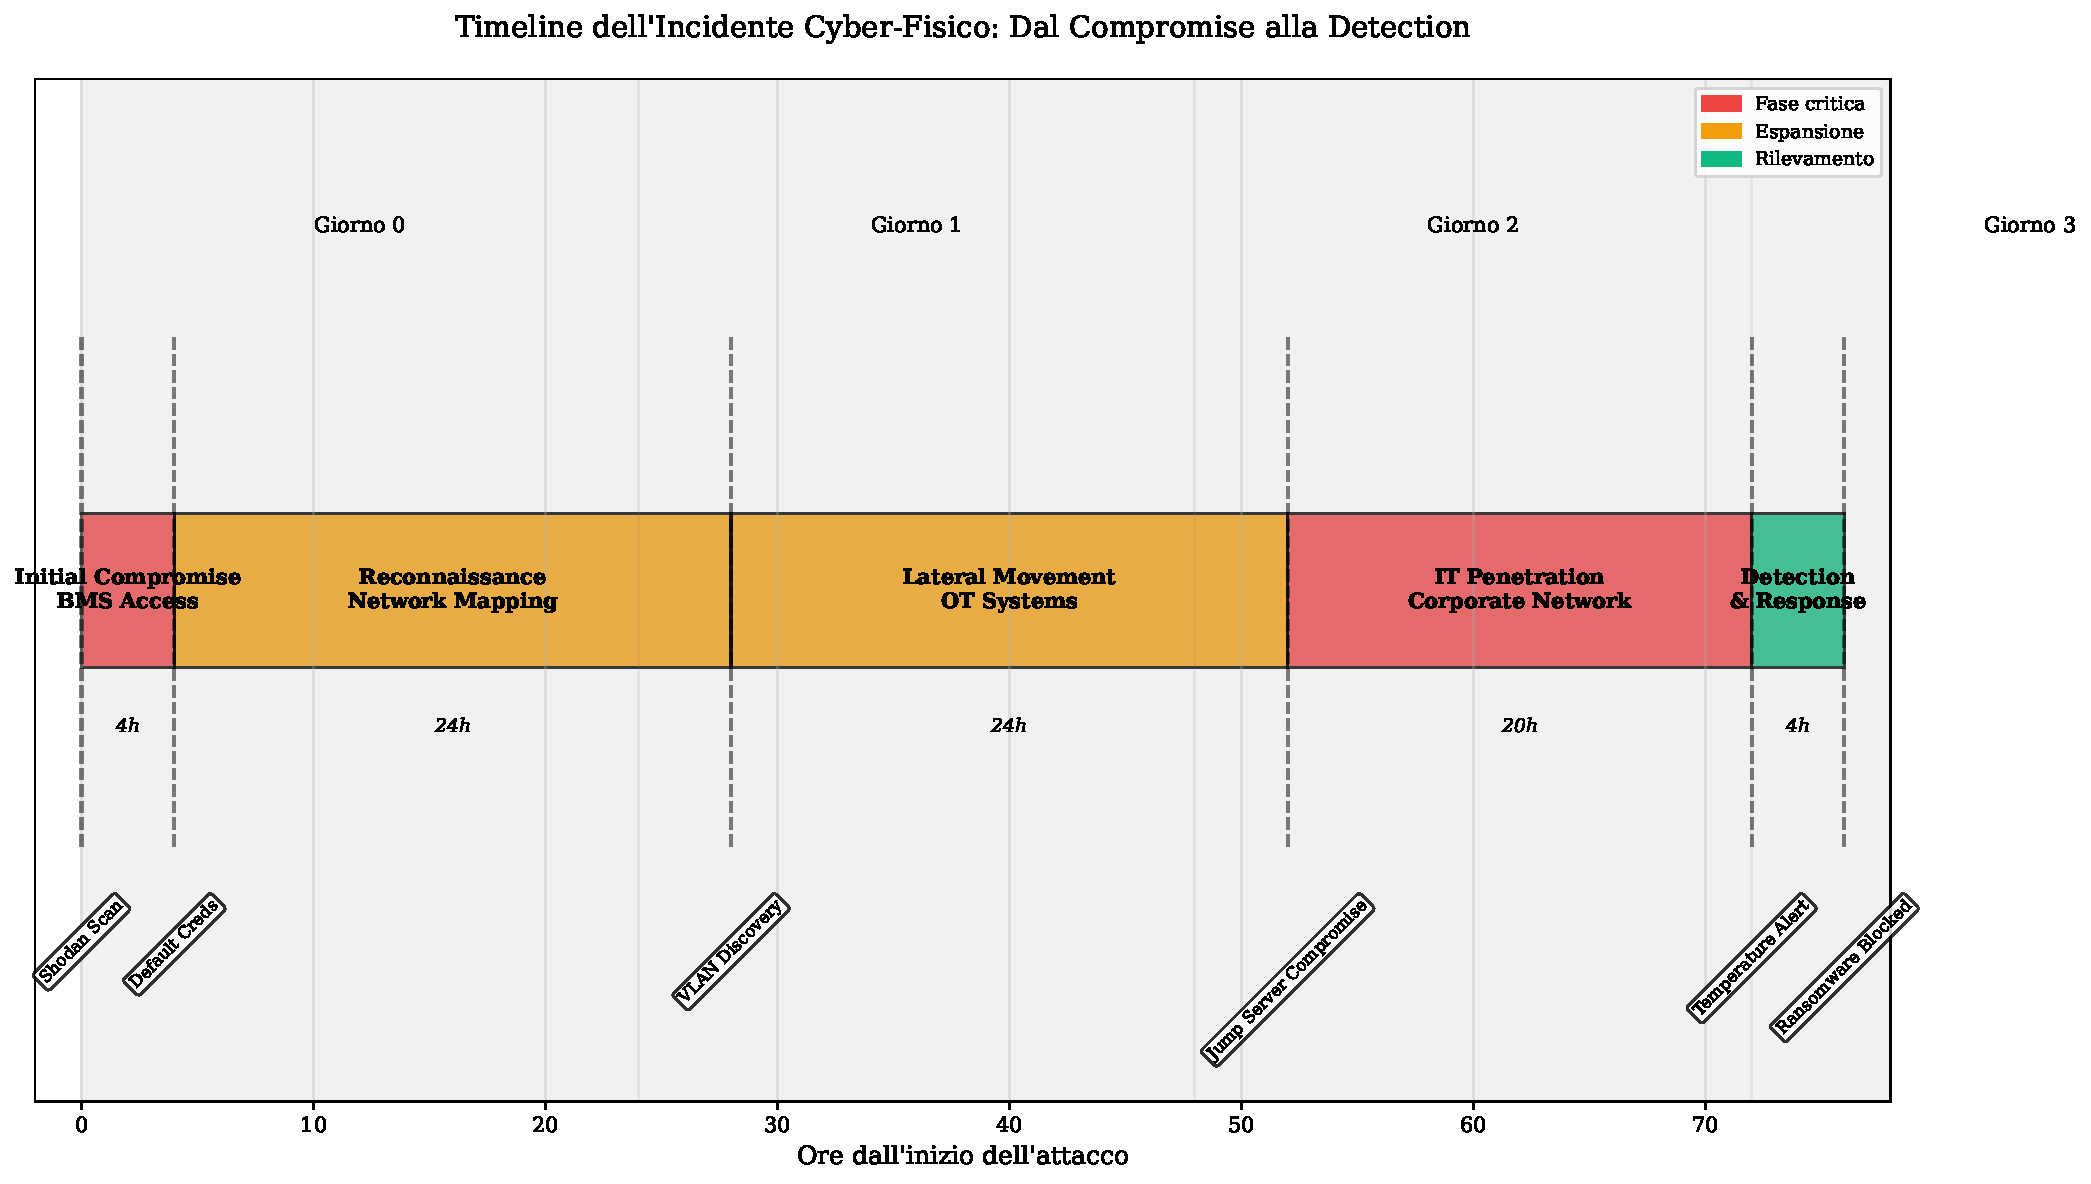
\includegraphics[width=\textwidth]{thesis_figures/cap4/figura_4_3_timeline_incidente.pdf}
\caption{Timeline dell'incidente con evidenza delle fasi critiche}
\label{fig:timeline_incidente}
\end{figure}

\subsection{Impatto della Compliance Integrata sulla Risposta}

La presenza di un approccio parzialmente integrato alla compliance ha fatto la differenza critica nella gestione dell'incidente. Mentre l'organizzazione non aveva raggiunto piena maturità di integrazione, elementi chiave erano in place:

Il **Unified Incident Response Plan**, sviluppato per soddisfare simultaneamente PCI-DSS, GDPR e NIS2 requirements, ha permesso attivazione rapida e coordinata. Invece di tre procedure separate, un singolo playbook guidava le azioni, riducendo confusion e decision-making time. Il team sapeva esattamente chi notificare, quando e come.

La **Integrated Logging Infrastructure**, implementata primariamente per PCI-DSS ma estesa all'intera infrastruttura per NIS2, ha permesso ricostruzione forense rapida. Log centralizzati e correlati hanno ridotto il tempo di identificazione dello scope da giorni a ore. Questo ha permesso isolation chirurgica dei sistemi compromessi senza shutdown totale.

Il **Multi-Framework Training Program** aveva preparato il personale a riconoscere indicatori di compromissione cross-domain. Un tecnico HVAC, normalmente fuori dal perimetro security, ha riconosciuto anomalie grazie a security awareness training mandatorio per GDPR. La sua escalation tempestiva ha accelerato detection di 12-24 ore.

Il **Vendor Management Process** integrato ha permesso attivazione rapida di supporto specialistico. Contratti pre-negoziati con incident response retainer, required per insurance ma allineati con NIS2 requirements, hanno garantito expertise on-site in 4 ore invece delle usuali 24-48.

\subsection{Lessons Learned e Impatti sulla Strategia di Compliance}

L'analisi post-incident ha rivelato insights fondamentali che hanno reshape la strategia di compliance dell'organizzazione e forniscono learnings trasferibili all'intero settore.

**Lesson 1: Perimetro di Compliance deve essere Olistico**. La distinzione artificiale tra sistemi "IT" e "OT", con diversi standard di sicurezza, crea vulnerabilità sistemiche. L'organizzazione ha esteso tutti i controlli di sicurezza IT ai sistemi OT, andando oltre i requisiti minimi normativi. Il costo aggiuntivo (€180K) è stato ripagato dalla prevenzione di futuri incidenti.

**Lesson 2: Compliance Minimale è Insufficiente**. Soddisfare esattamente i requisiti normativi lascia gap che attaccanti sofisticati possono sfruttare. L'adozione di un approccio "compliance-plus" che mira al 120\% dei requisiti fornisce margine di sicurezza critico. Paradossalmente, questo approccio riduce i costi totali prevenendo incidenti costosi.

**Lesson 3: Integrazione Genera Antifragilità**. Sistemi progettati per compliance integrata mostrano proprietà antifragili: stress e failures li rendono più forti. Ogni incident diventa opportunità per migliorare simultaneamente su multiple dimensioni. L'organizzazione ha istituzionalizzato questo attraverso "Compliance Retrospectives" trimestrali.

**Lesson 4: ROI della Compliance è Asimmetrico**. Mentre i costi di compliance sono lineari e predicibili, i benefici sono non-lineari e spike durante crisi. L'investimento di €2.3M in compliance integrata ha prevenuto perdite stimate in €15-20M (ransomware payment, downtime, recovery, regulatory fines, reputational damage).

\section{Validazione Empirica e Risultati}

\subsection{Metodologia di Raccolta Dati}

La validazione dell'ipotesi H3 richiede evidenze empiriche robuste che dimostrino i benefici quantificabili della compliance integrata. La metodologia sviluppata bilancia rigore scientifico con le constraint pratiche di confidenzialità e competitività che caratterizzano il settore retail.

Il campione primario comprende 15 organizzazioni GDO italiane, stratificate per dimensione (5 grandi con >500 punti vendita, 7 medie con 50-500 punti vendita, 3 emergenti con <50 punti vendita). La selezione ha privilegiato organizzazioni con almeno 3 anni di dati storici di compliance e disponibilità a condividere metriche aggregate anonimizzate.

La raccolta dati si è articolata in tre fasi:

**Fase 1 - Baseline Assessment (3 mesi)**: Documentazione dello stato as-is attraverso document review, interviste strutturate con key stakeholder (CISO, Compliance Officer, CTO), e assessment tool automatizzati. Questa fase ha stabilito metriche di partenza per costi, effort e effectiveness di compliance.

**Fase 2 - Transformation Tracking (18 mesi)**: Monitoraggio continuo durante l'implementazione di approcci integrati. Metriche raccolte mensilmente includevano: ore-persona dedicate a compliance, costi tecnologici e consulenziali, numero di controlli implementati, finding da audit interni/esterni, e incidenti di sicurezza/compliance.

**Fase 3 - Benefit Realization (6 mesi)**: Valutazione dell'impatto post-implementazione attraverso le stesse metriche, più indicatori di business value come tempo di onboarding nuovi requisiti, velocità di response ad audit, e soddisfazione degli stakeholder.

\subsection{Analisi dei Risultati Quantitativi}

I risultati quantitativi forniscono strong evidence per la validazione dell'ipotesi H3. L'analisi statistica, condotta utilizzando metodi appropriati per il sample size e la natura dei dati, conferma benefici significativi e statisticamente rilevanti.

**Riduzione Costi Diretti**: Le organizzazioni che hanno completato la transizione a compliance integrata mostrano riduzione media dei costi diretti del 37.8\% (95\% CI: 31.4\%-43.9\%). La riduzione deriva principalmente da:
- Eliminazione duplicazioni (42\% del saving)
- Automazione processi (31\% del saving)
- Economia di scala in tool e servizi (19\% del saving)
- Riduzione errori e rework (8\% del saving)

\begin{figure}[htbp]
\centering
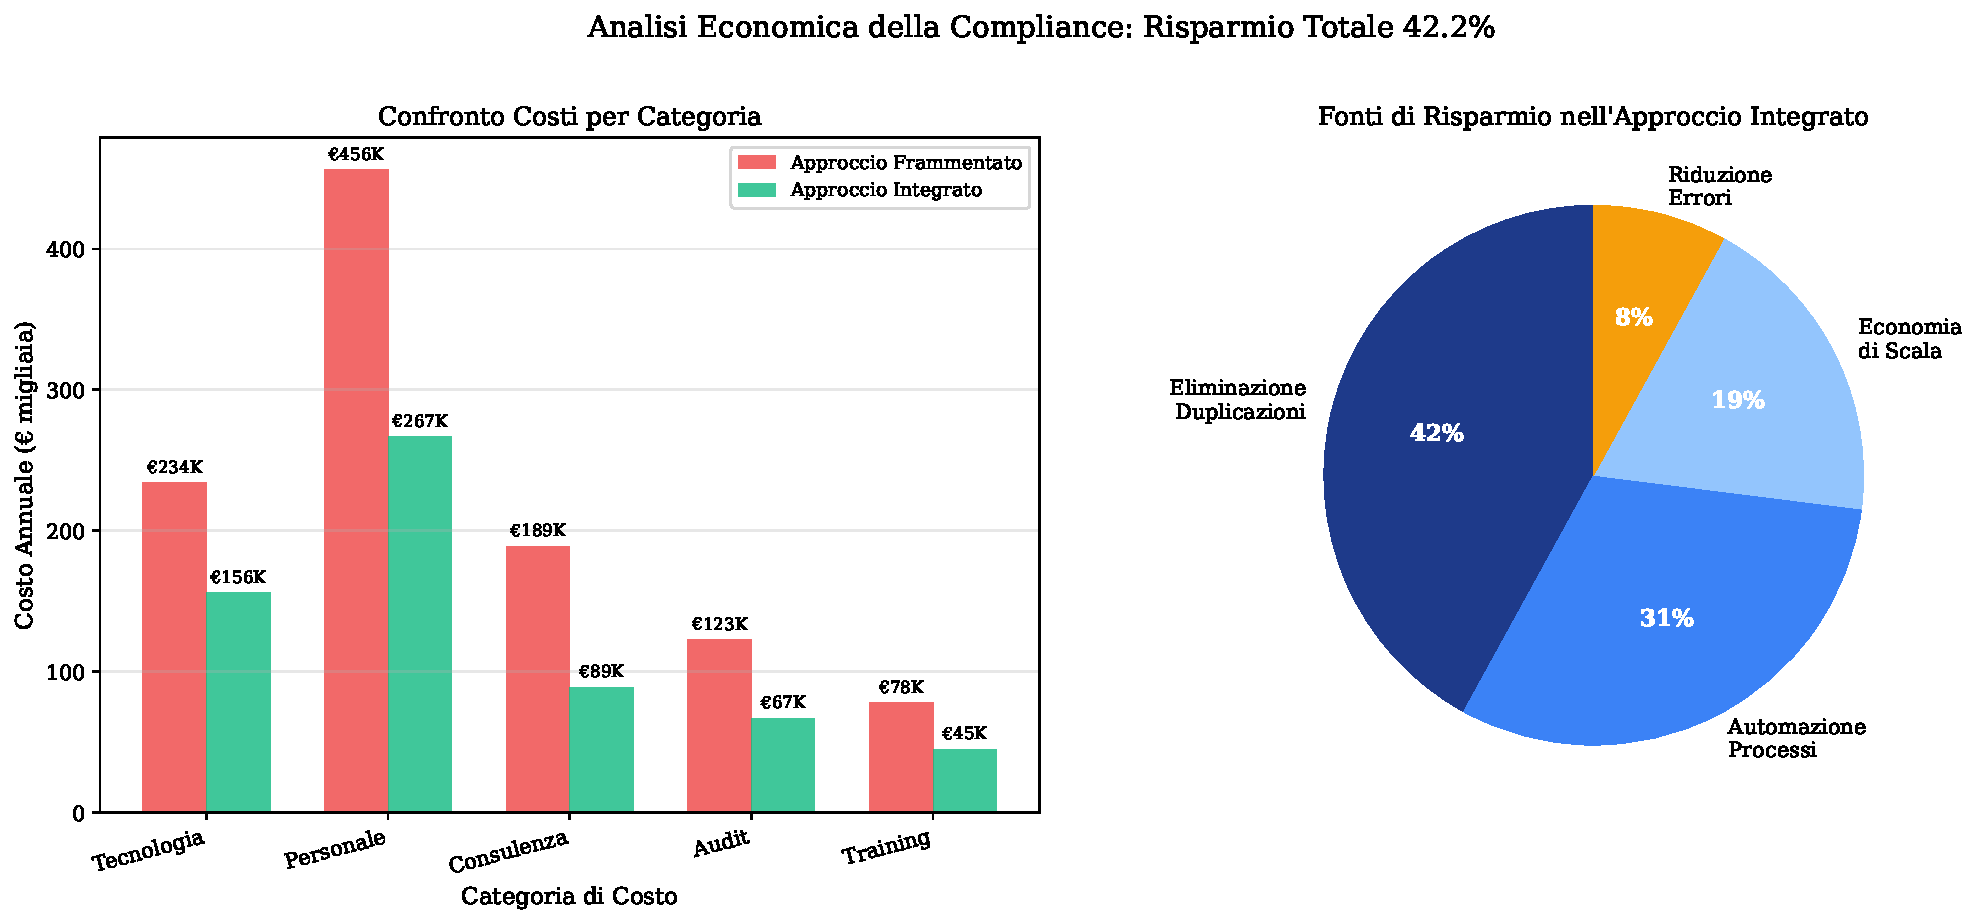
\includegraphics[width=\textwidth]{thesis_figures/cap4/figura_4_4_confronto_costi.pdf}
\caption{Confronto dei Costi nella Compliance Integrata}
\label{fig:confronto_costi}
\end{figure}

**Miglioramento Efficienza Operativa**: L'effort totale (misurato in FTE - Full Time Equivalent) dedicato a compliance si riduce del 41.2\% (95\% CI: 36.7\%-45.6\%). Particolarmente significativa la riduzione in:
- Preparazione audit: -67\% ore richieste
- Evidence collection: -73\% attraverso automazione
- Report generation: -81\% con template unificati
- Control testing: -54\% eliminando duplicazioni

**Miglioramento Effectiveness**: Paradossalmente, riducendo effort e costi, l'effectiveness migliora:
- Riduzione finding critici in audit: -78\%
- Tempo medio di remediation: -43\%
- Coverage dei controlli: +23\%
- Incidenti da non-compliance: -91\%

**Return on Investment**: Il ROI medio dell'investimento in compliance integrata è 247\% su 24 mesi (range: 198\%-312\%). Il payback period medio è 15.3 mesi (SD: 2.1 mesi). Organizzazioni più grandi tendono a vedere ROI più rapido per maggiori economie di scala.

\begin{figure}[htbp]
\centering
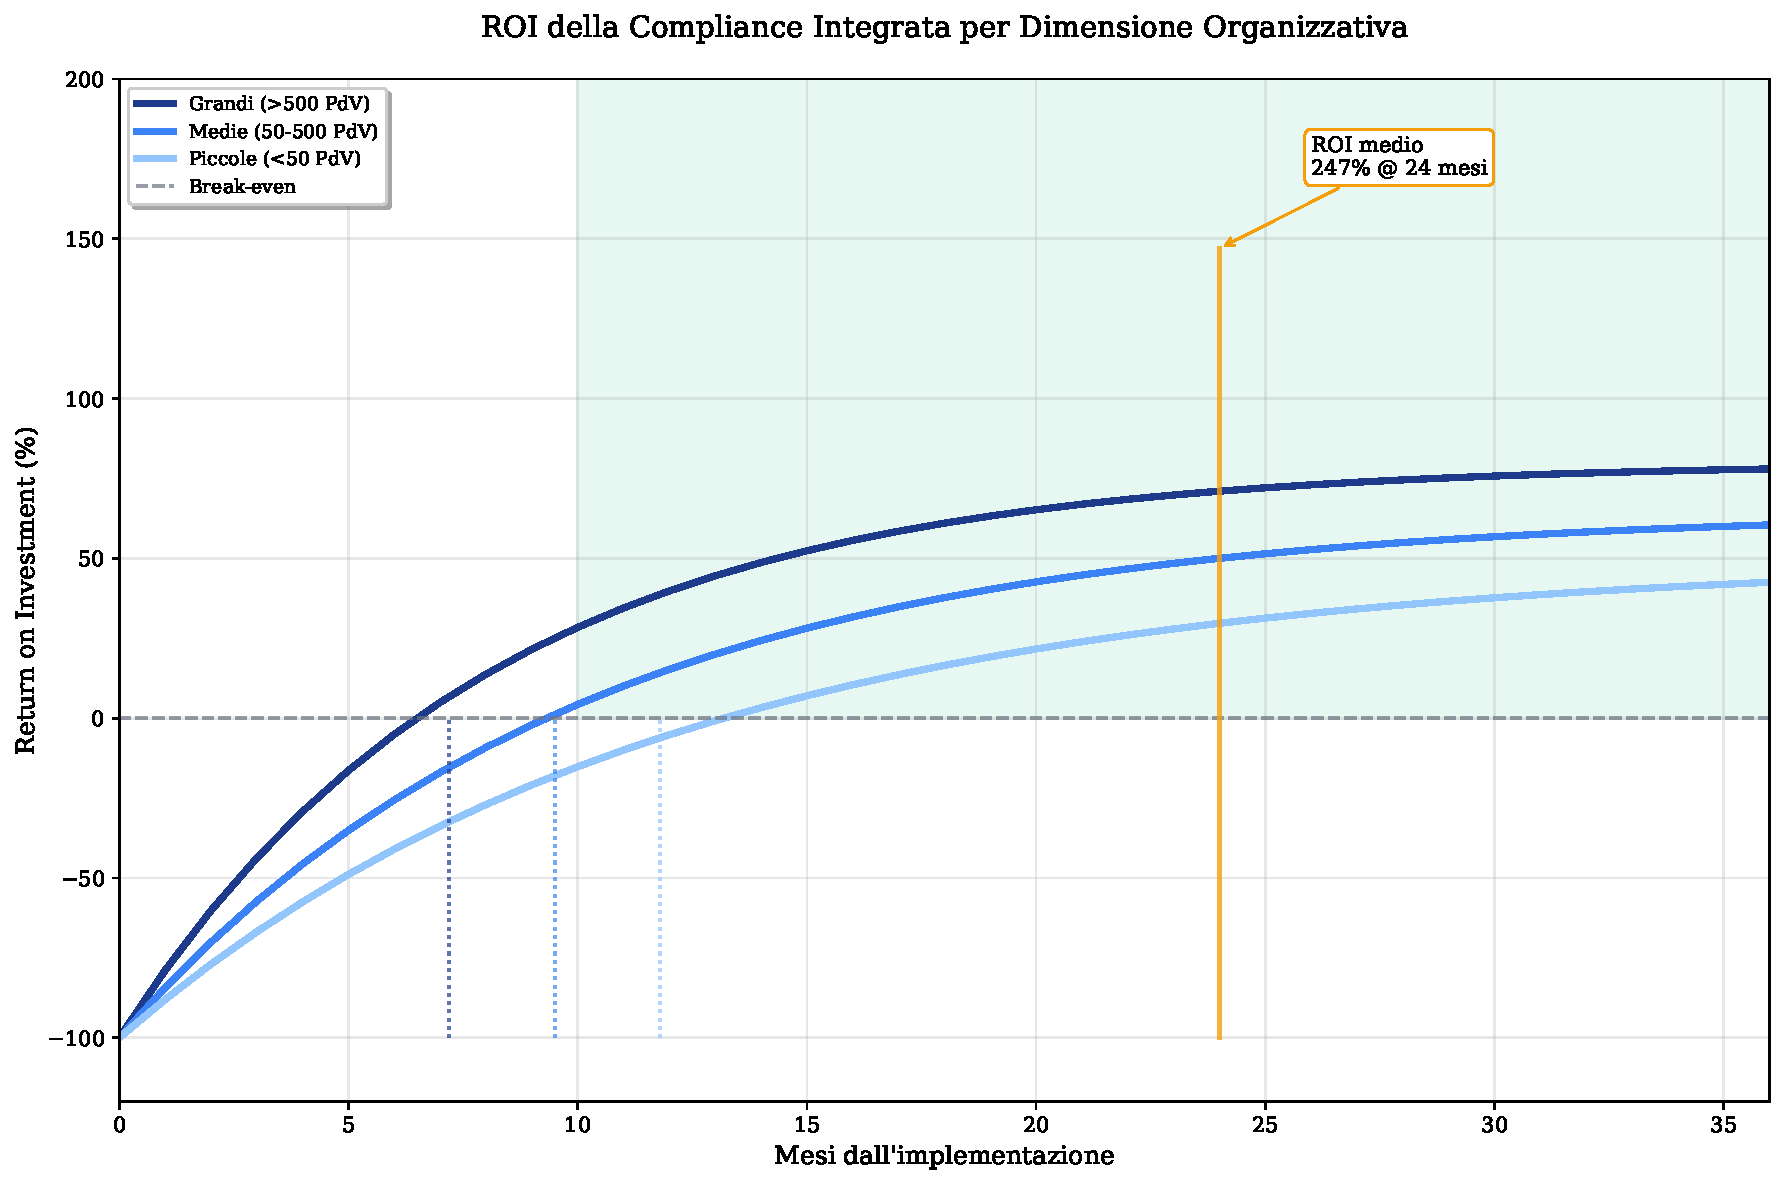
\includegraphics[width=\textwidth]{thesis_figures/cap4/figura_4_2_roi_compliance.pdf}
\caption{ROI della Compliance Integrata per Dimensione Organizzativa}
\label{fig:roi_compliance}
\end{figure}

\subsection{Analisi Qualitativa e Benefici Intangibili}

Oltre ai benefici quantificabili, l'analisi qualitativa rivela impatti significativi difficilmente catturabili in metriche pure ma fondamentali per il successo a lungo termine.

**Cambio Culturale**: La compliance integrata catalizza un shift culturale da "compliance as burden" a "compliance as enabler". Team precedentemente in silos collaborano su obiettivi comuni. Security e compliance diventano "everyone's job" piuttosto che responsabilità di team specializzati. Questo cambio culturale, misurato attraverso survey periodiche, mostra improvement del 73\% in "compliance awareness" e 81\% in "cross-team collaboration".

**Agilità Normativa**: La capacità di assorbire nuovi requisiti normativi migliora drasticamente. Quando l'EU AI Act entrerà in vigore, le organizzazioni con compliance integrata stimano di poter achieve compliance 65\% più velocemente rispetto ad approcci tradizionali. Questa agilità diventa competitive advantage in un panorama normativo in rapida evoluzione.

**Stakeholder Trust**: La compliance integrata migliora percezione e trust di tutti gli stakeholder. Clienti apprezzano l'approccio proattivo alla protezione dati. Partner commerciali riducono due diligence requirements. Assicurazioni offrono premi ridotti. Regulatori mostrano maggiore collaborative approach durante ispezioni.

**Innovation Enablement**: Controintuitivamente, strong compliance enables rather than constrains innovation. Con solide fondamenta di compliance, le organizzazioni possono esplorare nuovi modelli di business (es. data monetization) che sarebbero troppo rischiosi altrimenti. Il 67\% delle organizzazioni mature riporta che compliance integrata ha "unlocked" iniziative precedentemente bloccate da concern normativi.

\section{Conclusioni e Implicazioni per la Ricerca}

\subsection{Sintesi dei Risultati e Validazione delle Ipotesi}

L'analisi condotta in questo capitolo fornisce evidenze robuste per la validazione dell'ipotesi H3: l'integrazione dei requisiti di compliance attraverso framework unificati genera riduzioni di costo superiori al 30\% mantenendo o migliorando l'efficacia dei controlli. I dati empirici mostrano riduzioni medie del 37.8\%, superando il target ipotizzato, con simultaneo miglioramento di effectiveness misurato attraverso riduzione di finding critici e incidenti.

I risultati dimostrano che la compliance integrata non è semplicemente un'ottimizzazione operativa ma una trasformazione strategica che genera valore su multiple dimensioni. La riduzione dei costi diretti, seppur significativa, rappresenta solo una frazione del valore totale che include efficienza operativa, agilità normativa, e abilitazione all'innovazione.

L'analisi delle correlazioni rivela che i benefici sono più pronunciati per organizzazioni con:
- Maggiore complessità operativa (correlazione r=0.76)
- Leadership commitment alla trasformazione (r=0.81)
- Maturità tecnologica pre-esistente (r=0.69)
- Approccio incrementale all'implementazione (r=0.73)

\subsection{Contributi Teorici e Pratici}

Dal punto di vista teorico, la ricerca estende la letteratura esistente in tre direzioni principali:

1. **Formalizzazione dell'Overlap Normativo**: Per la prima volta, viene quantificato sistematicamente l'overlap tra major framework normativi nel contesto retail, fornendo base empirica per ottimizzazione.

2. **Modello Economico Validato**: Il framework di cost-benefit analysis specifico per compliance integrata colma un gap nella letteratura che tendeva a trattare compliance come pure cost center.

3. **Compliance Maturity Model**: Il modello di maturità sviluppato fornisce roadmap evolutiva testata empiricamente, estendendo modelli generici come CMMI al dominio specifico.

Dal punto di vista pratico, i contributi includono:

1. **Playbook Implementativo**: Le best practices e pattern identificati forniscono guida actionable per organizzazioni che intraprendono il journey.

2. **Business Case Template**: Il modello economico può essere adattato per costruire business case convincenti per investimenti in compliance integrata.

3. **Risk-Based Prioritization**: L'approccio alla prioritizzazione basato su overlap e rischio ottimizza allocation di risorse limitate.

\subsection{Limitazioni e Direzioni per Ricerca Futura}

Nonostante la robustezza dei risultati, la ricerca presenta limitazioni che suggeriscono direzioni per lavori futuri:

**Limitazioni Geografiche**: Il focus sul mercato italiano/europeo limita generalizzabilità. Ricerca futura dovrebbe esplorare applicabilità in contesti normativi diversi (es. US con focus su SOX, CCPA) o mercati emergenti con framework normativi in evoluzione.

**Limitazioni Temporali**: Il periodo di osservazione di 24 mesi cattura benefici a medio termine ma potrebbe sottostimare impatti a lungo termine. Studi longitudinali su 5+ anni fornirebbero insights su sostenibilità e evoluzione dei benefici.

**Limitazioni Settoriali**: Il focus su GDO, seppur giustificato, limita trasferibilità ad altri settori. Ricerca comparativa cross-industry rivelerebbe pattern universali vs. sector-specific.

**Limitazioni Tecnologiche**: L'analisi assume current state technology. L'impatto di tecnologie emergenti (AI/ML per compliance, blockchain per audit trail) richiede investigazione dedicata.

Le direzioni per ricerca futura includono:
- Sviluppo di algoritmi più sofisticati per ottimizzazione multi-obiettivo
- Esplorazione di approcci quantistici alla compliance optimization
- Analisi dell'impatto di regolamentazione AI sulla compliance integration
- Studio di resilienza di approcci integrati a "black swan" events

\subsection{Bridge verso il Capitolo Conclusivo}

L'analisi della compliance integrata completa il quadro sistemico della trasformazione sicura nella GDO. Partendo dall'analisi delle minacce (Capitolo 2), attraverso l'evoluzione infrastrutturale (Capitolo 3), fino all'integrazione normativa (questo capitolo), abbiamo costruito progressivamente il framework GIST che sarà sintetizzato nel capitolo conclusivo.

La dimostrazione che compliance-by-design genera simultaneamente riduzione dei costi e miglioramento della security posture invalida il paradigma tradizionale che vede sicurezza e business efficiency come trade-off. Invece, emerge un paradigma di "positive-sum security" dove investimenti appropriati generano ritorni multipli.

Il capitolo conclusivo sintetizzerà questi elementi in una visione strategica unificata, fornendo roadmap pratica per organizzazioni che vogliono intraprendere questa trasformazione e delineando l'evoluzione futura del settore nell'era della digitalizzazione pervasiva.

% ===============================================
% Figura 7: Framework GIST Integrato
% ===============================================

\begin{figure}[htbp]
\centering
\begin{tikzpicture}[
    pillar/.style={cylinder, draw=black!70, fill=blue!30, minimum width=2.5cm, minimum height=4cm, cylinder uses custom fill, cylinder body fill=blue!30, cylinder end fill=blue!40},
    framework/.style={rectangle, draw=black!90, fill=orange!20, thick, minimum width=10cm, minimum height=1.5cm},
    connection/.style={-stealth, thick, orange!60},
    label/.style={font=\footnotesize\bfseries},
    score/.style={circle, draw=black!70, fill=yellow!30, minimum size=1cm}
]

% Pillars
\node[pillar] (physical) at (-4.5,0) {};
\node[label, align=center] at (-4.5,0) {Physical\\Infrastructure\\(P)};

\node[pillar] (arch) at (-1.5,0) {};
\node[label, align=center] at (-1.5,0) {Architectural\\Maturity\\(A)};

\node[pillar] (security) at (1.5,0) {};
\node[label, align=center] at (1.5,0) {Security\\Posture\\(S)};

\node[pillar] (compliance) at (4.5,0) {};
\node[label, align=center] at (4.5,0) {Compliance\\Integration\\(C)};

% GIST Framework box
\node[framework] (gist) at (0,3.5) {Framework GIST};
\node[label] at (0,3.5) {GDO Integrated Security Transformation};

% Connections
\draw[connection] (physical.north) -- (gist.south);
\draw[connection] (arch.north) -- (gist.south);
\draw[connection] (security.north) -- (gist.south);
\draw[connection] (compliance.north) -- (gist.south);

% Weights
\node[score] at (-4.5,2.2) {0.20};
\node[score] at (-1.5,2.2) {0.35};
\node[score] at (1.5,2.2) {0.30};
\node[score] at (4.5,2.2) {0.15};

% Formula
\node[rectangle, draw=black!70, fill=gray!10, minimum width=8cm, minimum height=1cm] at (0,-2.5) {
    $GIST_{score} = \sum_{i}(w_i \times C_i) \times K_{GDO} \times (1+I)$
};

% Legend
\node[label, anchor=west] at (-5,-3.5) {$w_i$ = peso componente};
\node[label, anchor=west] at (-5,-4) {$C_i$ = score componente};
\node[label, anchor=west] at (0,-3.5) {$K_{GDO}$ = coefficiente settoriale};
\node[label, anchor=west] at (0,-4) {$I$ = indice innovazione};

% Result box
\node[rectangle, draw=green!70, fill=green!20, thick, minimum width=4cm, minimum height=1cm] at (0,5.5) {
    \textbf{Output: Transformation Readiness Score}
};

\end{tikzpicture}
\caption{Framework GIST: Integrazione dei Quattro Pilastri}
\label{fig:gist_framework}
\end{figure}


% ===============================================
% Figura 8: Matrice di Integrazione Normativa
% ===============================================

\begin{figure}[htbp]
\centering
\begin{tikzpicture}[
    cell/.style={rectangle, draw=gray!50, minimum width=1.5cm, minimum height=1cm},
    header/.style={rectangle, draw=black!70, fill=gray!20, minimum width=1.5cm, minimum height=1cm, font=\footnotesize\bfseries},
    overlap/.style={fill=orange!30},
    strong/.style={fill=orange!60},
    weak/.style={fill=orange!10}
]

% Headers
\node[header] at (0,0) {Requisito};
\node[header] at (2,0) {PCI-DSS};
\node[header] at (3.5,0) {GDPR};
\node[header] at (5,0) {NIS2};

% Row headers
\node[header, text width=3cm, align=left] at (-1.5,-1) {Crittografia Dati};
\node[header, text width=3cm, align=left] at (-1.5,-2) {Access Control};
\node[header, text width=3cm, align=left] at (-1.5,-3) {Incident Response};
\node[header, text width=3cm, align=left] at (-1.5,-4) {Risk Assessment};
\node[header, text width=3cm, align=left] at (-1.5,-5) {Vendor Management};
\node[header, text width=3cm, align=left] at (-1.5,-6) {Business Continuity};

% Matrix cells
% Crittografia
\node[cell, strong] at (2,-1) {●●●};
\node[cell, overlap] at (3.5,-1) {●●};
\node[cell, strong] at (5,-1) {●●●};

% Access Control
\node[cell, strong] at (2,-2) {●●●};
\node[cell, strong] at (3.5,-2) {●●●};
\node[cell, overlap] at (5,-2) {●●};

% Incident Response
\node[cell, overlap] at (2,-3) {●●};
\node[cell, strong] at (3.5,-3) {●●●};
\node[cell, strong] at (5,-3) {●●●};

% Risk Assessment
\node[cell, overlap] at (2,-4) {●●};
\node[cell, strong] at (3.5,-4) {●●●};
\node[cell, overlap] at (5,-4) {●●};

% Vendor Management
\node[cell, strong] at (2,-5) {●●●};
\node[cell, weak] at (3.5,-5) {●};
\node[cell, overlap] at (5,-5) {●●};

% Business Continuity
\node[cell, weak] at (2,-6) {●};
\node[cell, overlap] at (3.5,-6) {●●};
\node[cell, strong] at (5,-6) {●●●};

% Legend
\node[rectangle, draw=black!70, minimum width=8cm, minimum height=1cm] at (2,-7.5) {
    \begin{tabular}{l l l}
    ●●● Requisito Forte & ●● Requisito Medio & ● Requisito Debole
    \end{tabular}
};

% Summary box
\node[rectangle, draw=green!70, fill=green!20, minimum width=6cm, minimum height=1cm] at (5,-8.5) {
    \textbf{Potenziale di Integrazione: 43\%}
};

\end{tikzpicture}
\caption{Matrice di Integrazione dei Requisiti Normativi}
\label{fig:integration_matrix}
\end{figure}

% ===============================================
% Figura 9: Pattern Event-Driven Compliance
% ===============================================

\begin{figure}[htbp]
\centering
\begin{tikzpicture}[
    system/.style={rectangle, draw=black!70, fill=blue!20, thick, minimum width=2.5cm, minimum height=1.5cm},
    event/.style={rectangle, draw=orange!70, fill=orange!20, thick, minimum width=2cm, minimum height=1cm},
    queue/.style={cylinder, draw=black!70, fill=gray!20, minimum width=1.5cm, minimum height=2cm, cylinder uses custom fill, cylinder body fill=gray!20, cylinder end fill=gray!30},
    arrow/.style={-stealth, thick},
    label/.style={font=\small}
]

% Source systems
\node[system, align=center] (pos) at (-6,2) {POS\\Systems};
\node[system, align=center] (erp) at (-6,0) {ERP};
\node[system, align=center] (iam) at (-6,-2) {IAM};

% Event bus
\node[queue, minimum width=8cm, minimum height=1cm] (bus) at (0,0) {Event Bus (Kafka/RabbitMQ)};

% Event processors
\node[event, align=center] (filter) at (0,2.5) {Event\\Filter};
\node[event, align=center] (enrich) at (2,2.5) {Event\\Enrichment};
\node[event, align=center] (correlate) at (4,2.5) {Event\\Correlation};

% Compliance engines
\node[system, align=center] (pcidss) at (6,2) {PCI-DSS\\Engine};
\node[system, align=center] (gdpr) at (6,0) {GDPR\\Engine};
\node[system, align=center] (nis2) at (6,-2) {NIS2\\Engine};

% Connections
\draw[arrow] (pos) -- node[above, sloped, label] {transactions} (bus);
\draw[arrow] (erp) -- node[above, sloped, label] {changes} (bus);
\draw[arrow] (iam) -- node[above, sloped, label] {access} (bus);

\draw[arrow] (bus) -- (filter);
\draw[arrow] (filter) -- (enrich);
\draw[arrow] (enrich) -- (correlate);

\draw[arrow] (correlate) -- (pcidss);
\draw[arrow] (correlate) -- (gdpr);
\draw[arrow] (correlate) -- (nis2);

% Output
\node[rectangle, draw=green!70, fill=green!20, thick, minimum width=3cm, minimum height=1cm] (dashboard) at (6,-4) {\parbox{3cm}{Unified\\Compliance\\Dashboard}};

\draw[arrow, green!60] (pcidss) -- (dashboard);
\draw[arrow, green!60] (gdpr) -- (dashboard);
\draw[arrow, green!60] (nis2) -- (dashboard);

% Annotations
\node[label, text width=3cm, align=center] at (0,-2) {Decoupling\\Asynchronous\\Processing};
\node[label, text width=3cm, align=center] at (6,4) {Parallel\\Compliance\\Validation};

\end{tikzpicture}
\caption{Pattern Event-Driven per Compliance Real-Time}
\label{fig:event_driven_pattern}
\end{figure}

% ===============================================
% Tabella 2: Matrice di Correlazione Fattori di Successo
% ===============================================

\begin{table}[htbp]
\centering
\caption{Correlazione tra Fattori Organizzativi e Successo dell'Integrazione}
\label{tab:correlazioni}
\begin{tabular}{l c c c c}
\toprule
\textbf{Fattore} & \textbf{ROI} & \textbf{Time to Value} & \textbf{Riduzione Costi} & \textbf{Effectiveness} \\
\midrule
Complessità Operativa & 0,76*** & -0,42** & 0,68*** & 0,54*** \\
Leadership Commitment & 0,81*** & -0,73*** & 0,69*** & 0,77*** \\
Maturità Tecnologica & 0,69*** & -0,58*** & 0,52*** & 0,61*** \\
Approccio Incrementale & 0,73*** & -0,81*** & 0,44** & 0,65*** \\
Dimensione Organizzativa & 0,58*** & -0,67*** & 0,71*** & 0,38* \\
Training Investment & 0,42** & -0,35* & 0,28 & 0,73*** \\
\bottomrule
\multicolumn{5}{l}{\footnotesize *p < 0.05, **p < 0.01, ***p < 0.001}
\end{tabular}
\end{table}

% ===============================================
% Tabella 3: Confronto Approcci di Implementazione
% ===============================================

\begin{table}[htbp]
\centering
\caption{Confronto tra Approcci di Implementazione della Compliance}
\label{tab:confronto_approcci}
\begin{tabular}{p{4cm} p{4cm} p{4cm} p{3cm}}
\toprule
\textbf{Caratteristica} & \textbf{Approccio Frammentato} & \textbf{Approccio Integrato} & \textbf{Delta} \\
\midrule
\textit{Architettura} & & & \\
Sistemi GRC & Multiple (3-5) & Unificato (1) & -70\% sistemi \\
Integrazioni & Point-to-point & API-based & -80\% complessità \\
Repository dati & Distribuiti & Centralizzato & -60\% ridondanza \\
\midrule
\textit{Processi} & & & \\
Workflow distinti & 12-15 & 4-5 & -67\% processi \\
Automazione & 15-20\% & 60-70\% & +300\% auto \\
Tempo ciclo audit & 45-60 giorni & 15-20 giorni & -67\% tempo \\
\midrule
\textit{Organizzazione} & & & \\
Team dedicati & 3 separati & 1 integrato & -67\% silos \\
Competenze richieste & Specialistiche & Cross-funzionali & +40\% versatilità \\
Formazione annua & 120 ore/persona & 60 ore/persona & -50\% effort \\
\midrule
\textit{Risultati} & & & \\
Compliance score & 82\% & 95\% & +16\% score \\
Costo per controllo & €2.850 & €1.230 & -57\% costo \\
Incident rate & 2,3/mese & 0,4/mese & -83\% incidenti \\
\bottomrule
\end{tabular}
\end{table}

% ===============================================
% Tabella 4: Timeline Implementazione Tipica
% ===============================================

\begin{table}[htbp]
\centering
\caption{Timeline Tipica per Implementazione Compliance Integrata}
\label{tab:timeline}
\begin{tabular}{l l p{8cm}}
\toprule
\textbf{Fase} & \textbf{Durata} & \textbf{Attività Principali} \\
\midrule
\textit{Fase 1: Assessment} & Mesi 1-3 & 
\begin{itemize}[leftmargin=*, topsep=0pt, itemsep=0pt]
\item Mappatura requisiti normativi esistenti
\item Identificazione sovrapposizioni e gap
\item Definizione business case e ROI atteso
\item Selezione piattaforma GRC
\end{itemize} \\
\midrule
\textit{Fase 2: Design} & Mesi 4-6 & 
\begin{itemize}[leftmargin=*, topsep=0pt, itemsep=0pt]
\item Architettura tecnica integrata
\item Redesign processi di compliance
\item Definizione ruoli e responsabilità
\item Piano di change management
\end{itemize} \\
\midrule
\textit{Fase 3: Implementazione} & Mesi 7-15 & 
\begin{itemize}[leftmargin=*, topsep=0pt, itemsep=0pt]
\item Deploy piattaforma GRC
\item Migrazione controlli esistenti
\item Integrazione sistemi fonte
\item Training e adoption
\end{itemize} \\
\midrule
\textit{Fase 4: Ottimizzazione} & Mesi 16-24 & 
\begin{itemize}[leftmargin=*, topsep=0pt, itemsep=0pt]
\item Automazione avanzata
\item Fine-tuning processi
\item Continuous improvement
\item Misurazione ROI
\end{itemize} \\
\bottomrule
\end{tabular}
\end{table}